\documentclass[class=article]{standalone}

\begin{document}
	\section{Il Sistema}
	Il sistema è costituito da una bicicletta da un sensore.
	
	\begin{figure}[h]
	\begin{subfigure}[h]{0.5\textwidth}
		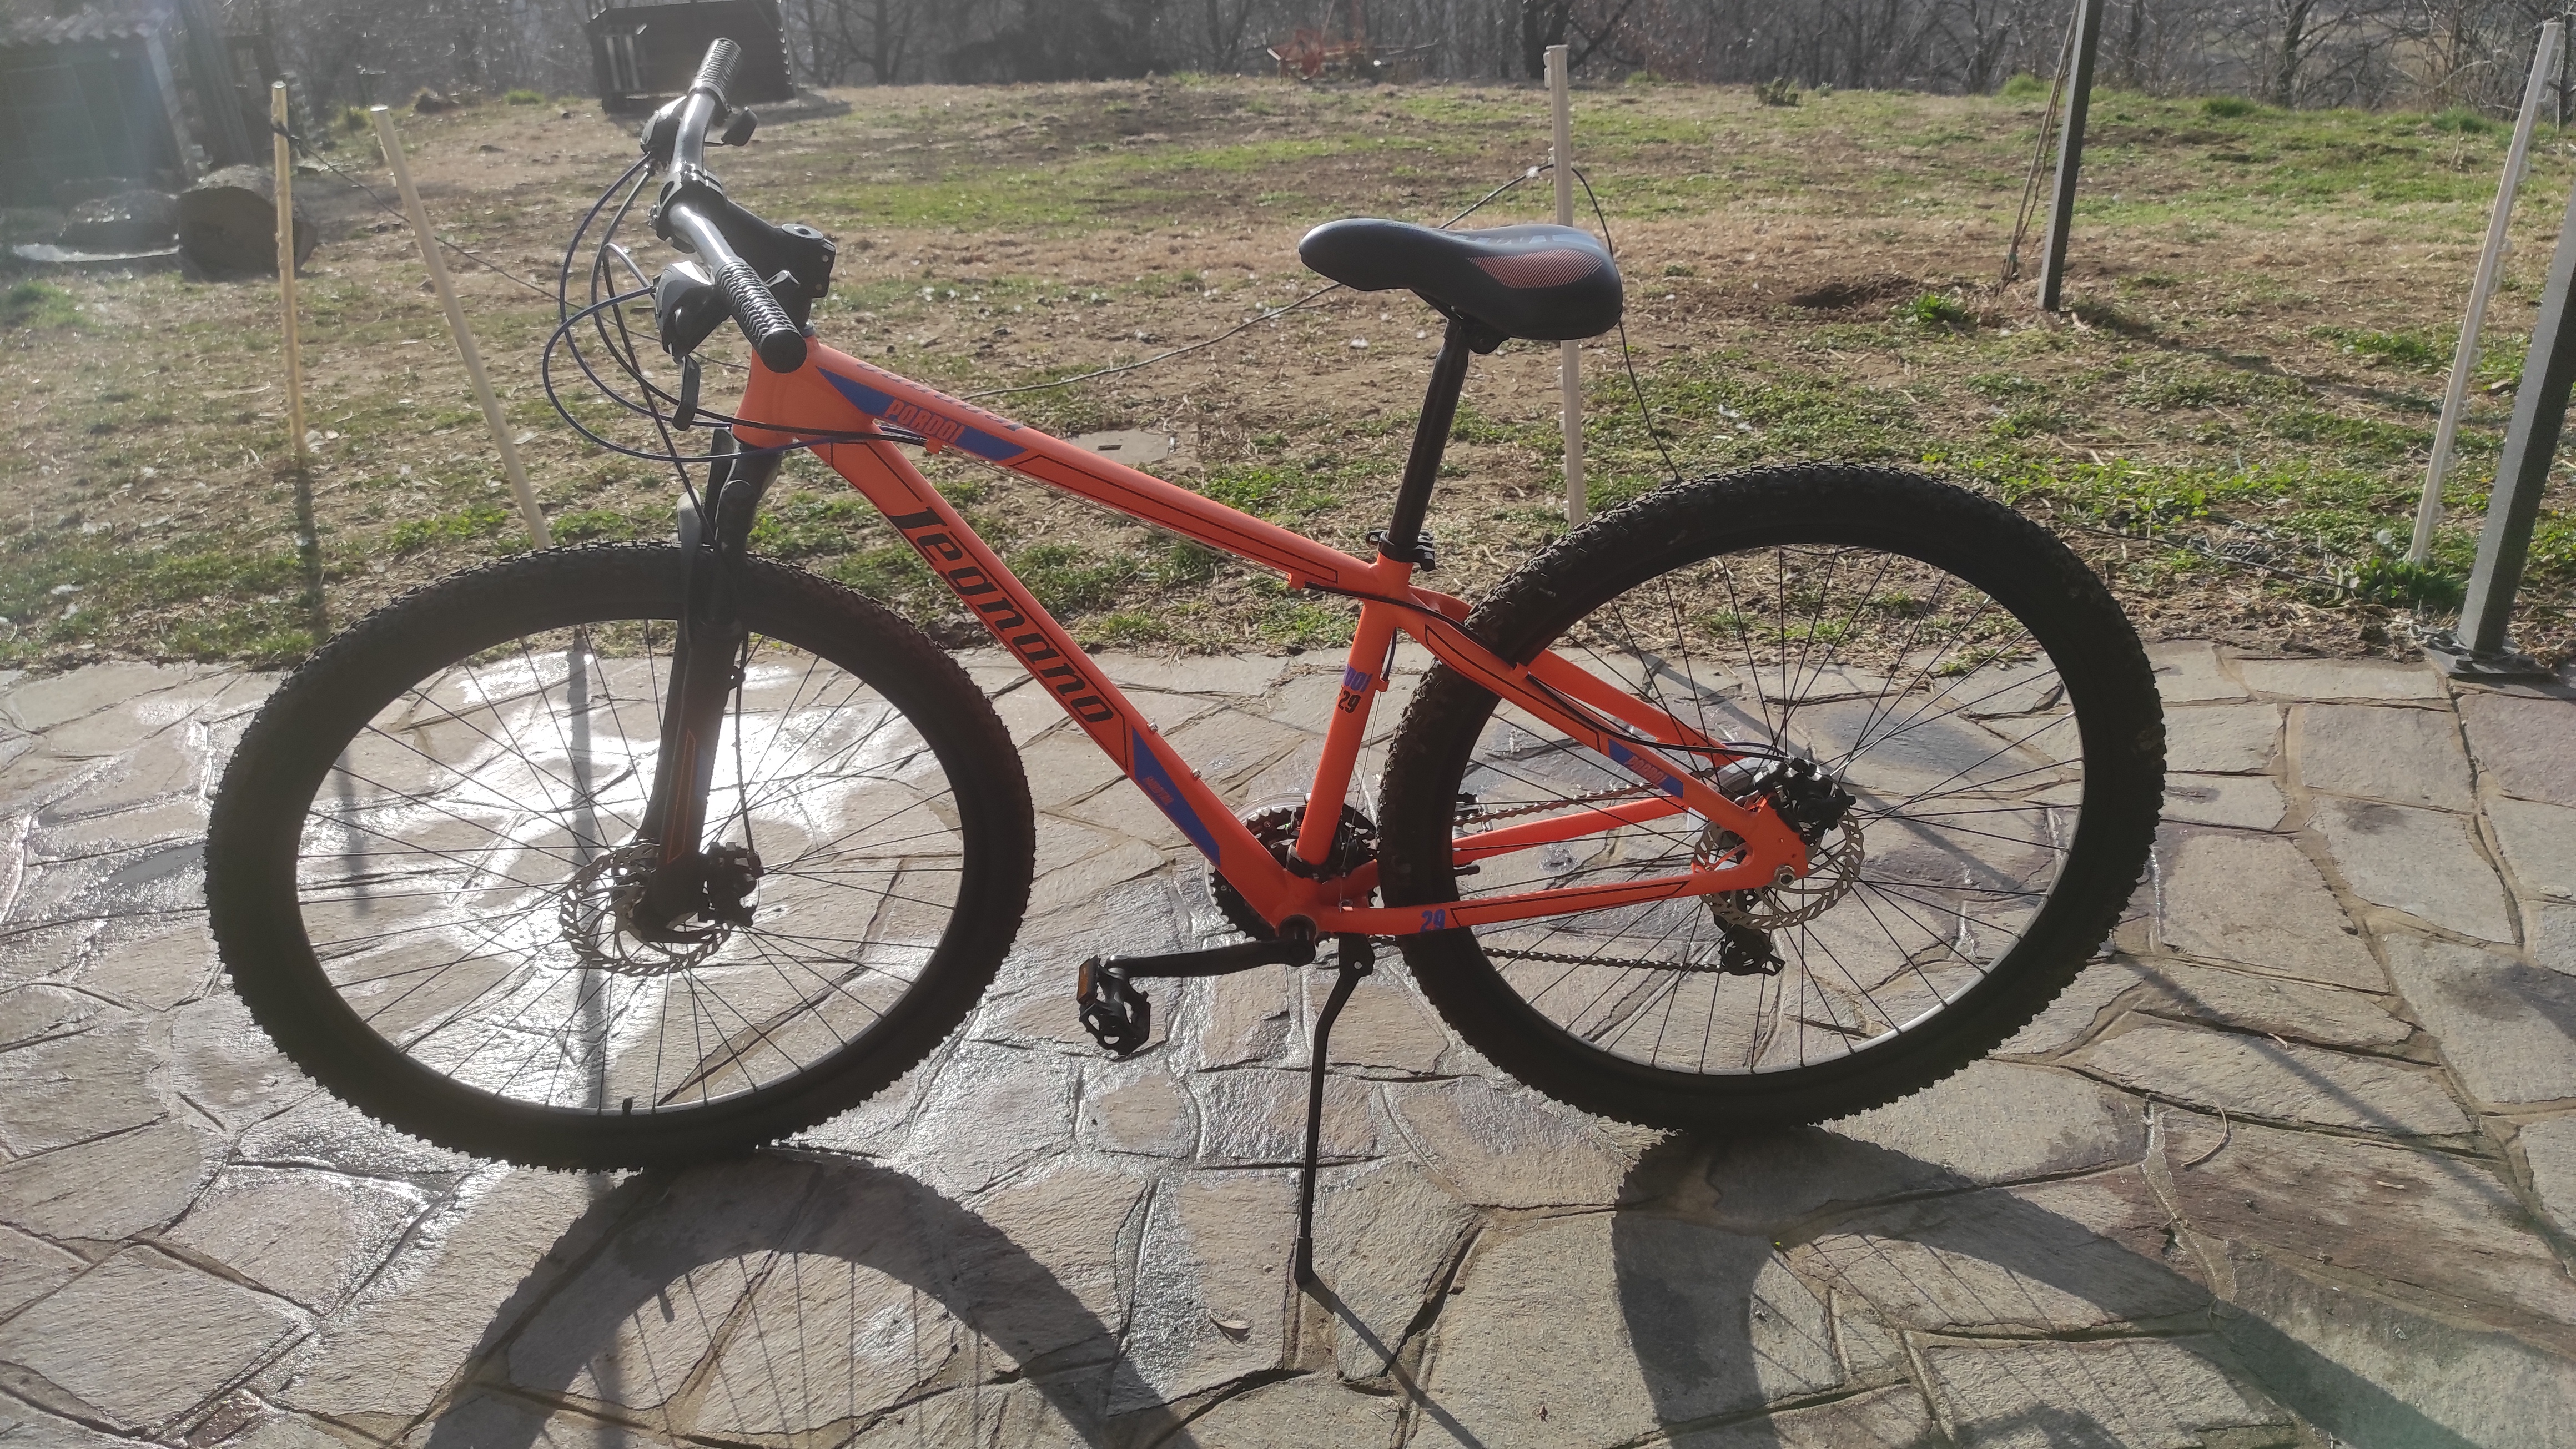
\includegraphics[width=0.9\linewidth]{./img/bicicletta2.jpg}
		\caption{}
		\label{fig:bici}
	\end{subfigure}
	\hfill
	\begin{subfigure}[h]{0.5\textwidth}
		\includegraphics[width=0.8\linewidth]{./img/bluecoin.jpg}
		\caption{}
		\label{fig:sensore}
	\end{subfigure}
	
	\caption[width=0.5\textwidth]{La bicicletta \ref{fig:bici} e il sensore \ref{fig:sensore} usati durante le uscite per acquisire i dati}
	\end{figure}
	
	\subsection{Sensore}
	Il sensore utilizzato è il Blue Coin della ST Microelettronics (\url{https://www.st.com/en/evaluation-tools/steval-bcnkt01v1.html}) sulla quale è stato montato il software di valutazione dello stesso STSW-BCNKT01 presente sulla pagina del sito del produttore che è, al momento della stesura, alla versione 2.4.0.
	
	Il sensore utilizzato è dotato di accelerometro, giroscopio, magnetometro, barometro, sensore di temperatura e microfono. Nello svolgimento di questa tesi sono stati utilizzati solo i sensori di accelerazione, velocità angolare e campo magnetico in quanto sufficienti per ottenere i risultati da noi cercati.
	
	Interessante potrebbe essere l'introduzione del sensore di pressione per identificare quando la bicicletta si muove in salita o in discesa.
	
	Data la struttura della bicicletta, il sensore è stato montato su un'asse inclinato rispetto al piano parallelo al suolo. Questo ha causato la necessità di ruotare i dati dell'accelerometro al fine di portare il vettore gravità perpendicolare al suolo e di far coincidere il sistema di riferimento del sensore con quello della bicicletta.
	
	
\end{document}